\documentclass[aspectratio=169,11pt]{beamer}
\usetheme{metropolis}
\metroset{block=fill, sectionpage=progressbar, numbering=fraction, progressbar=frametitle}

\usepackage{fontspec}
\setsansfont{Segoe UI}
\setmonofont{Consolas}
\usepackage{fvextra}
\usepackage{booktabs}
\usepackage{xcolor}

% ---- Palette (mềm, học thuật) ----
\definecolor{deepteal}{HTML}{264653}
\definecolor{coral}{HTML}{E76F51}
\definecolor{tealc}{HTML}{2A9D8F}
\definecolor{cream}{HTML}{FBF9F5}
\definecolor{ink}{HTML}{233038}

\setbeamercolor{normal text}{fg=ink, bg=cream}
\setbeamercolor{frametitle}{fg=deepteal, bg=cream}     % không thanh màu chói
\setbeamercolor{title separator}{fg=coral}
\setbeamercolor{progress bar}{fg=coral}
\setbeamercolor{alerted text}{fg=coral}
\setbeamercolor{example text}{fg=tealc}
\setbeamercolor{itemize item}{fg=coral}
\setbeamercolor{itemize subitem}{fg=tealc}
\setbeamercolor{block title}{bg=tealc!18, fg=deepteal}
\setbeamercolor{block body}{bg=tealc!7}
\setbeamercolor{block title alerted}{bg=coral!20, fg=coral!60!black}
\setbeamercolor{block body alerted}{bg=coral!8}
\setbeamercolor{block title example}{bg=deepteal!12, fg=deepteal}
\setbeamercolor{block body example}{bg=deepteal!5}

\newcommand{\promptbox}[2]{\VerbatimInput[breaklines=true,breakanywhere=true,%
  breaksymbolleft={},breakautoindent=true,%
  fontsize=#1,baselinestretch=0.92,frame=single,framesep=4pt,%
  rulecolor=\color{deepteal!35},formatcom=\color{ink}]{#2}}
\newcommand{\take}[1]{\vfill{\footnotesize\color{deepteal}#1}}

\title{Tác nhân LLM trong trò chơi rủi ro tập thể}
\subtitle{Tái lập Milinski et al.\ (2008): prompt · kết quả · cơ chế}
\date{\today}
\author{Báo cáo nghiên cứu}

\begin{document}
\maketitle

% ======================================================================
\section{Bối cảnh}

\begin{frame}{Trò chơi rủi ro tập thể (Milinski 2008)}
  \begin{columns}[T]
    \begin{column}{0.57\textwidth}
      \textbf{Luật chơi}
      \begin{itemize}
        \item 6 người chơi, mỗi người vốn 40.
        \item 10 vòng; mỗi vòng đóng \{0, 2, 4\} vào quỹ chung.
        \item \alert{Mục tiêu nhóm}: tổng $\geq 120$.
        \item Không đạt $\Rightarrow$ với xác suất rủi ro $p$ cả nhóm \alert{mất sạch}; đạt thì giữ phần chưa đóng.
        \item Rủi ro $p \in \{0.9,\ 0.5,\ 0.1\}$.
      \end{itemize}
    \end{column}
    \begin{column}{0.40\textwidth}
      \textbf{Người thật làm gì?}
      \smallskip
      \begin{center}
      \begin{tabular}{cc}
        \toprule
        Rủi ro & Tỉ lệ đạt \\
        \midrule
        0.9 & 50\% \\
        0.5 & 10\% \\
        0.1 & \phantom{0}0\% \\
        \bottomrule
      \end{tabular}
      \end{center}
      \smallskip
      {\footnotesize Người \alert{hợp tác nhiều hơn khi rủi ro cao} — nhạy với rủi ro.}
    \end{column}
  \end{columns}
\end{frame}

\begin{frame}{Bốn điều kiện, ba mô hình}
  \begin{center}\small
  \begin{tabular}{lll}
    \toprule
    Điều kiện & Thao tác & So với baseline \\
    \midrule
    \textbf{1. Baseline} & (đối chứng)   & xem trọn lịch sử, trung tính \\
    \textbf{2. Memory}   & trí nhớ       & chỉ vòng gần nhất + sổ tay (giống paper) \\
    \textbf{3. Framing}  & khung tâm lý  & thêm khung "chỉ quan tâm tiền của bạn" \\
    \textbf{4. Persona}  & tính cách     & thêm 0$\to$6 tác nhân "ích kỷ" \\
    \bottomrule
  \end{tabular}
  \end{center}
  \vfill
  \begin{block}{Ba mô hình mã nguồn mở}
    \centering Qwen2.5-7B \quad•\quad Llama-3.1-8B \quad•\quad Gemma-2-9B \\
    {\footnotesize Mỗi điều kiện: 3 mức rủi ro $\times$ \{EN, VN\} $\times$ 10 lần lặp; quyết định đồng thời, ẩn danh, không giao tiếp.}
  \end{block}
\end{frame}

% ======================================================================
\section{1 · Baseline}

\begin{frame}[fragile]{Baseline — prompt ví dụ (vòng 3, đã có lịch sử)}
  \promptbox{\fontsize{7}{8}\selectfont}{prompt_baseline_r3.txt}
\end{frame}

\begin{frame}{Baseline — phớt lờ rủi ro (so với người)}
  \centering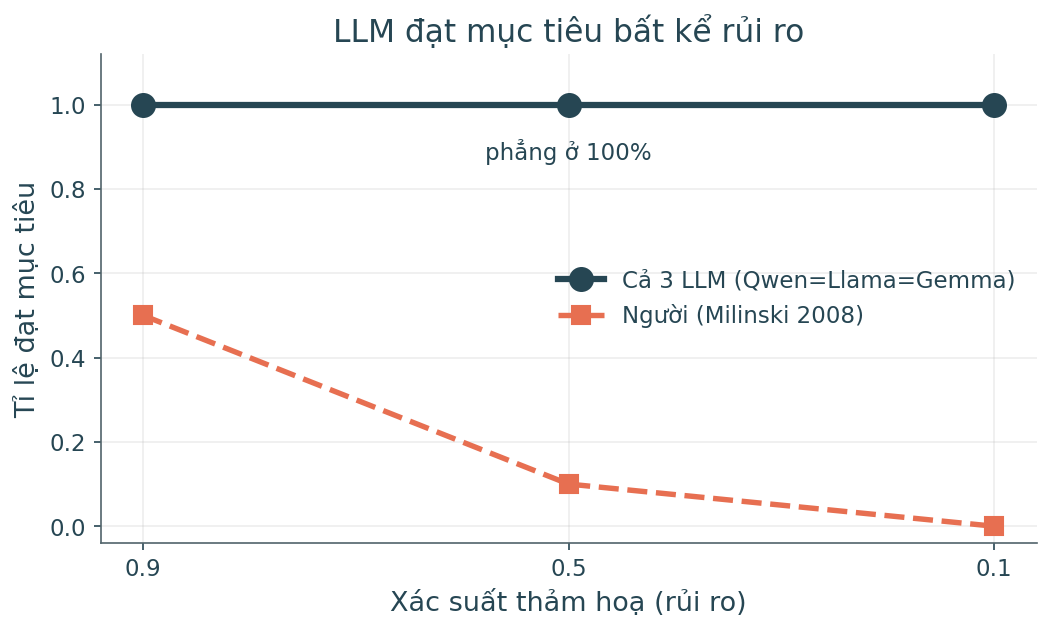
\includegraphics[height=0.70\textheight]{figs/A_reach_vs_risk.png}
  \take{Cả 3 mô hình đạt mục tiêu $\sim$100\% ở mọi mức rủi ro; người giảm 50$\to$10$\to$0\%.}
\end{frame}

\begin{frame}{Baseline — đóng góp cũng phẳng, chỉ khác độ hào phóng}
  \centering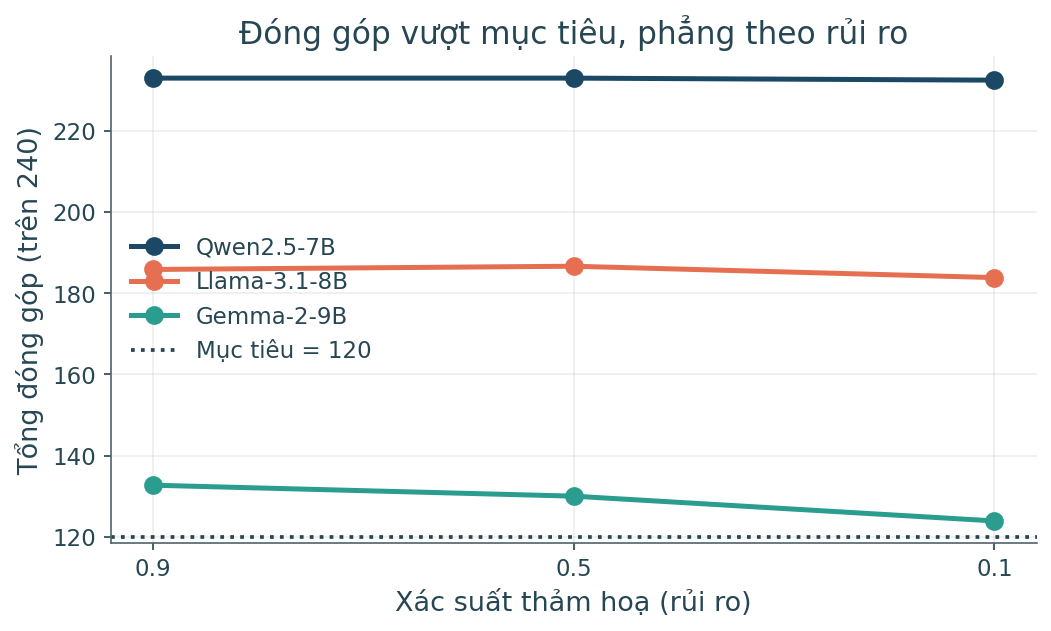
\includegraphics[height=0.66\textheight]{figs/B_contrib_vs_risk.png}
  \take{Mức đóng góp không phản ứng với rủi ro; thứ bậc hào phóng Qwen ($\sim$233) $>$ Llama ($\sim$185) $>$ Gemma ($\sim$129, sát mục tiêu nhất).}
\end{frame}

\begin{frame}{Baseline — “vân tay” lựa chọn của mỗi mô hình}
  \centering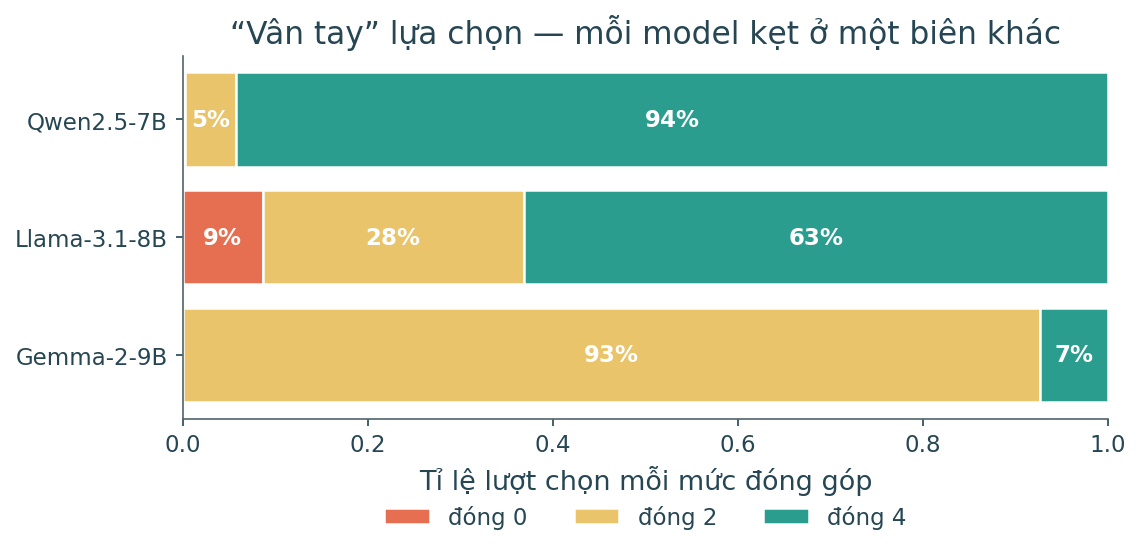
\includegraphics[height=0.64\textheight]{figs/H_choice_dist.png}
  \take{Qwen gần như luôn chọn 4 (94\%, kịch trần), Gemma khoá ở 2 (93\%, kịch sàn), chỉ Llama trộn cả ba $\Rightarrow$ Llama là thước đo nhạy nhất; hai model kia bị kiểm duyệt ở hai biên.}
\end{frame}

\begin{frame}{Baseline — “vân tay” tách theo 3 mức rủi ro}
  \centering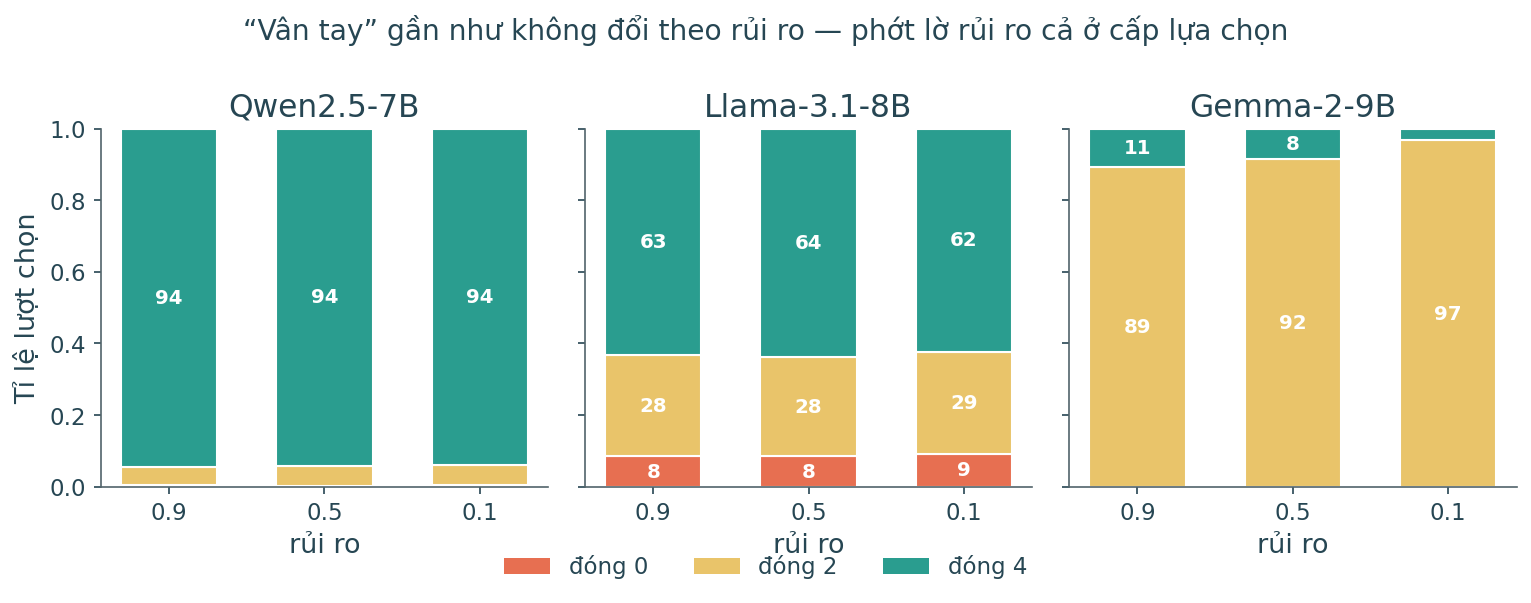
\includegraphics[height=0.62\textheight]{figs/H2_choice_dist_risk.png}
  \take{Phân phối lựa chọn gần như đứng yên qua rủi ro (Qwen 94/94/94, Llama 63/64/62) — phớt lờ rủi ro \emph{cả ở cấp lựa chọn}. Ghi chú nhỏ: chỉ Gemma hé một vệt đúng hướng (chọn 4: 3\%$\to$11\% khi rủi ro tăng), nhưng quá yếu để dịch reach.}
\end{frame}

\begin{frame}{Baseline — ngôn ngữ: tiếng Anh vs tiếng Việt}
  \centering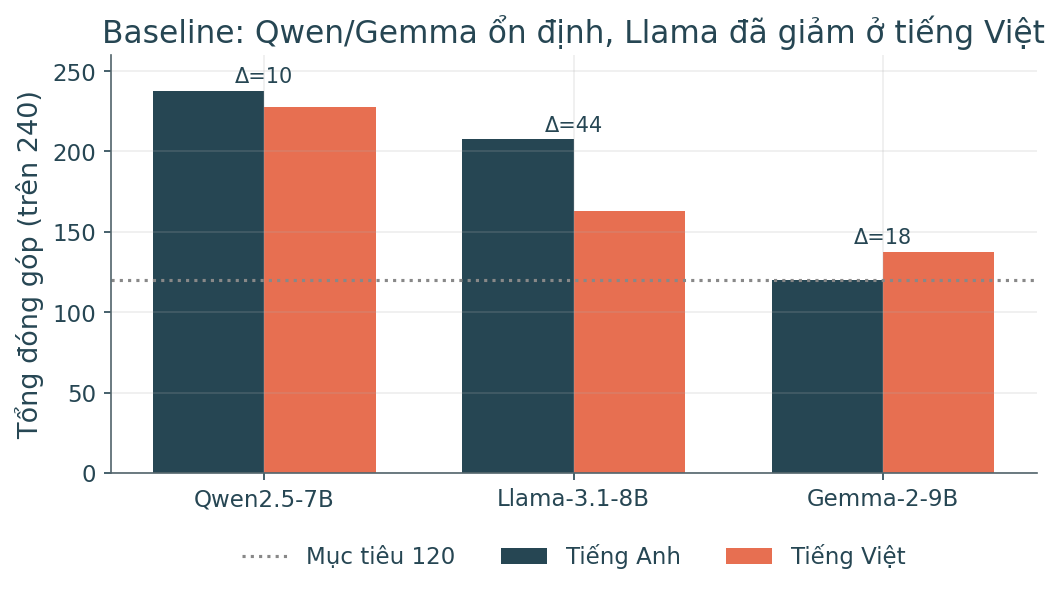
\includegraphics[height=0.66\textheight]{figs/I_lang_baseline.png}
  \take{Ở reach thì EN $=$ VN (đều 100\%); nhưng mức đóng góp đã hé trục ngôn ngữ — Llama giảm $\sim$44 đơn vị ở tiếng Việt, Qwen/Gemma gần như không đổi.}
\end{frame}

\begin{frame}{Baseline — hợp tác TĂNG dần (ngược người)}
  \centering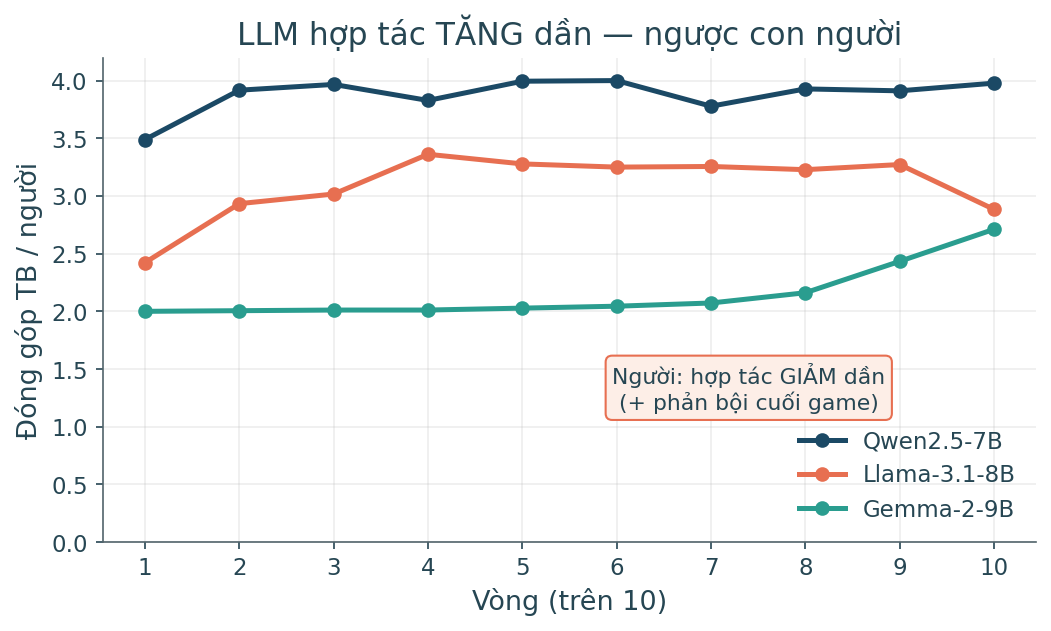
\includegraphics[height=0.66\textheight]{figs/C_round_dynamics.png}
  \take{Người: hợp tác giảm + phản bội cuối game. LLM: tăng dần rồi bão hoà, không phản bội.}
\end{frame}

% ======================================================================
\section{2 · Memory}

\begin{frame}{Memory — vì sao? (theo paper gốc)}
  \begin{itemize}
    \item Bản gốc KHÔNG cho xem trọn lịch sử / tổng tích luỹ — người chơi \textbf{tự ghi bằng giấy–bút}.
    \item Baseline (full history) là bản tiện-lợi-hoá; \alert{điều kiện scratchpad mới trung thành với paper}.
  \end{itemize}
  \vfill
  \begin{exampleblock}{Trích Milinski et al.\ (2008), PNAS — \emph{Materials and Methods}}
    \small\itshape
    ``\dots the cumulative sum of contributions was not displayed on the computer screen. Instead, the students were given pen and paper, and they were encouraged to take notes during the game.''
    \par\smallskip
    ``After each of 10 rounds, the decisions of the six subjects were displayed \dots each subject's decision was listed in the same position after each round \dots; thus, individual players were not anonymous within the game.''
  \end{exampleblock}
\end{frame}

\begin{frame}[fragile]{Memory — prompt (phần khác baseline)}
  \promptbox{\scriptsize}{delta_memory.txt}
\end{frame}

\begin{frame}{Memory — chỉ Gemma bị ảnh hưởng}
  \centering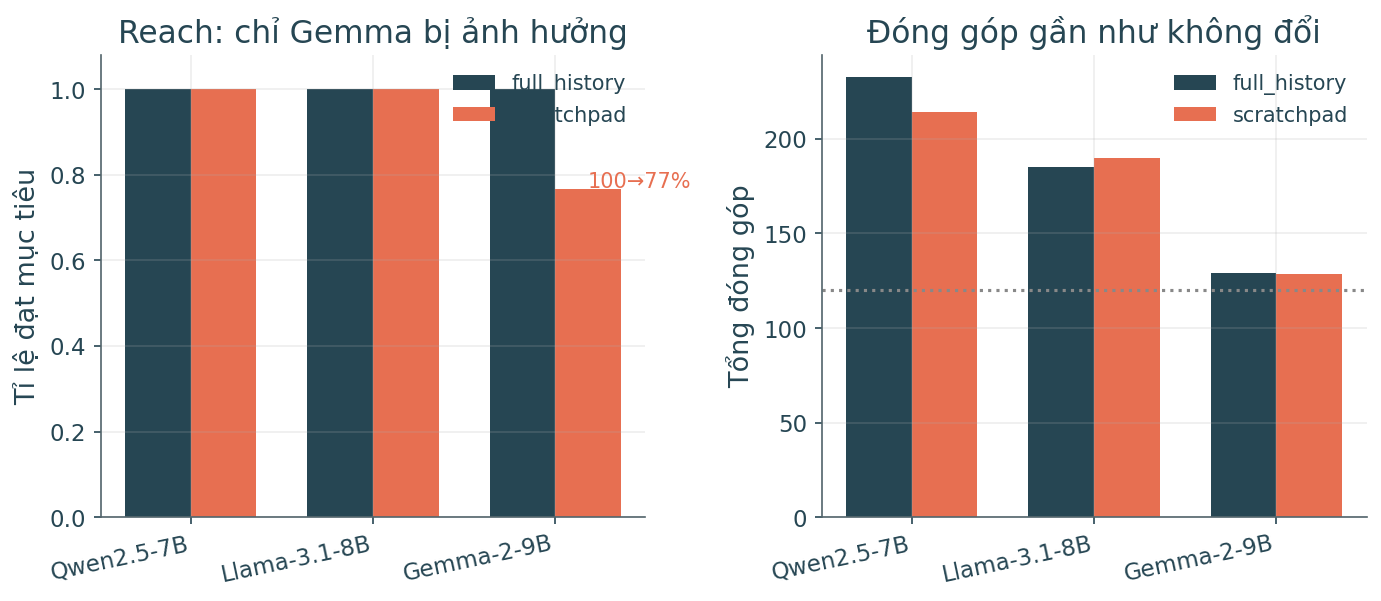
\includegraphics[height=0.66\textheight]{figs/M_memory.png}
  \take{Trí nhớ giới hạn chỉ hại model "sát mục tiêu" nhất (Gemma 100$\to$77\%); Llama/Qwen dư slack nên không sao.}
\end{frame}

\begin{frame}{Memory — động lực vòng: full-history vs scratchpad}
  \centering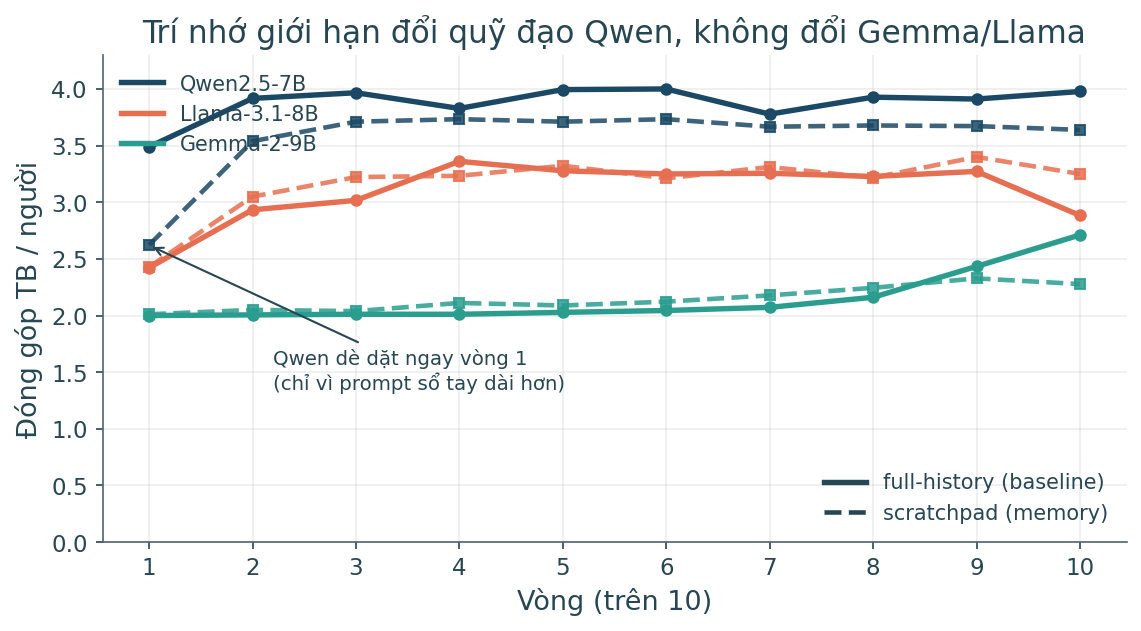
\includegraphics[height=0.66\textheight]{figs/M2_memory_dynamics.png}
  \take{Cùng game-state ở vòng 1, riêng Qwen dè dặt hơn dưới scratchpad (3.49$\to$2.62) chỉ vì phần hướng dẫn sổ tay dài thêm $\sim$554 ký tự; Gemma/Llama gần như giữ nguyên quỹ đạo.}
\end{frame}

% ======================================================================
\section{3 · Framing}

\begin{frame}[fragile]{Framing — khác baseline ở đâu?}
  \begin{block}{Thao tác — thiết kế 2$\times$2 (framing $\times$ memory)}
    {\footnotesize Chèn \textbf{khung tâm lý ích kỷ} lên đầu prompt; luật chơi giữ NGUYÊN. Khung này chạy trên \textbf{CẢ HAI} chế độ trí nhớ: full-history (như baseline) \emph{và} scratchpad (như memory) — so với neutral tương ứng.}
  \end{block}
  \promptbox{\scriptsize}{delta_framing.txt}
\end{frame}

\begin{frame}{Framing — \emph{giảm bao nhiêu} đóng góp (mạnh hơn ở tiếng Việt)}
  \centering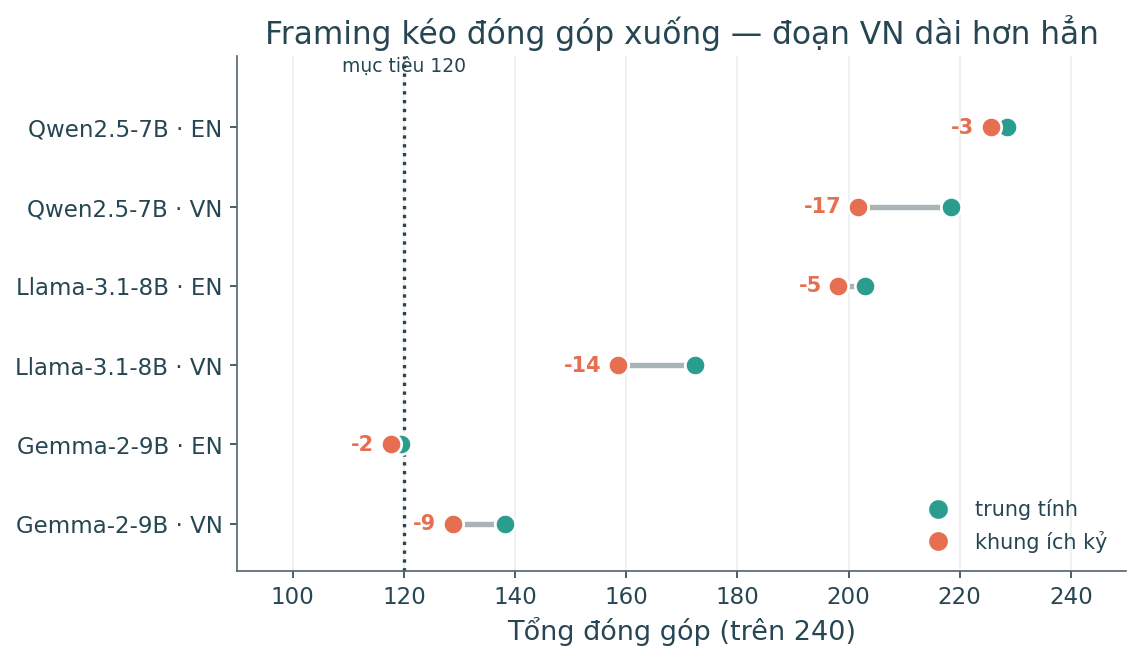
\includegraphics[height=0.66\textheight]{figs/FR_framing.png}
  \take{Khung ích kỷ kéo đóng góp xuống ở cả 3 model; mức giảm ở tiếng Việt lớn hơn tiếng Anh 2.9–5.8 lần.}
\end{frame}

\begin{frame}{Framing — \emph{ai hỏng} mục tiêu (tỉ lệ đạt: chỉ Gemma rớt)}
  \centering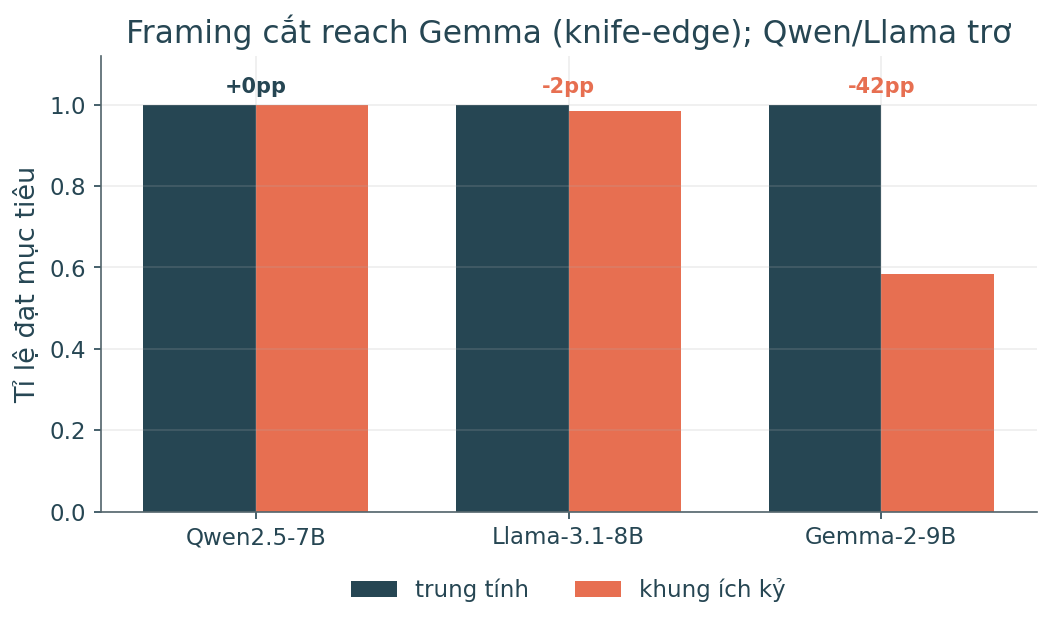
\includegraphics[height=0.66\textheight]{figs/FR3_framing_reach.png}
  \take{Cùng khung ích kỷ: Gemma rớt reach 100$\to$58\% ($-42$pp) vì chơi ngay trên vạch 120; Qwen/Llama gần như trơ — "dễ tổn thương" đo bằng khoảng cách tới ngưỡng, không phải mức đóng góp.}
\end{frame}

% ======================================================================
\section{4 · Persona}

\begin{frame}[fragile]{Persona — khác baseline ở đâu?}
  \begin{block}{Thao tác}
    {\footnotesize Gán cho mỗi tác nhân một \textbf{dòng tính cách}. Nhóm trộn 0$\to$6 tác nhân ích kỷ (gradient), vị trí xáo trộn. Phần còn lại như baseline.}
  \end{block}
  \promptbox{\scriptsize}{delta_persona.txt}
\end{frame}

\begin{frame}{Persona — thao tác hiệu quả nhất}
  \centering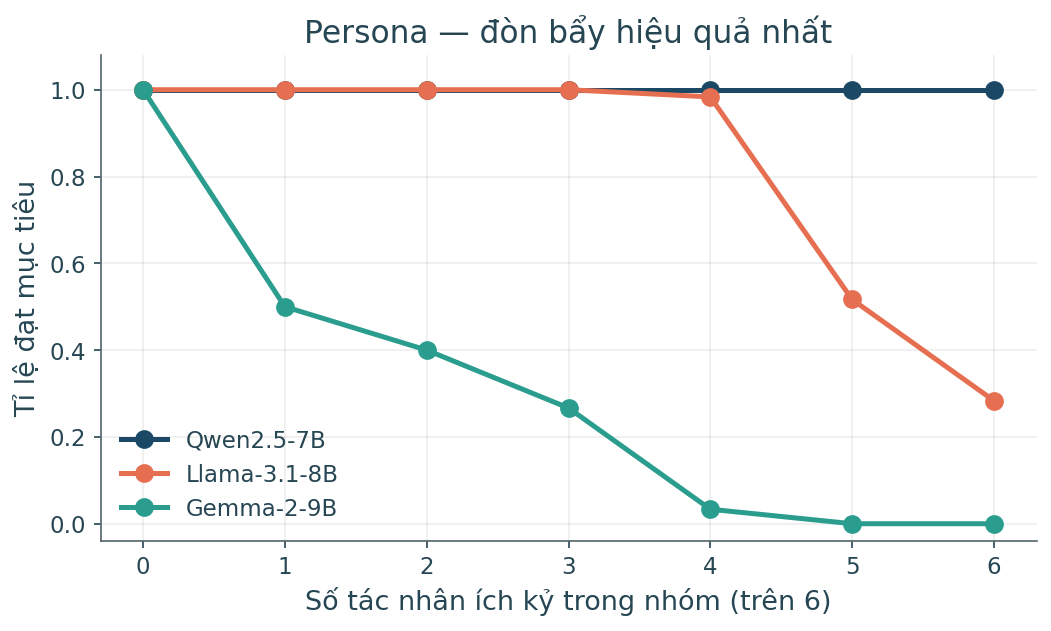
\includegraphics[height=0.66\textheight]{figs/D_persona_reach.png}
  \take{Gemma sụp ngay ở 1 tác nhân ích kỷ; Llama "vực thẳm" muộn; Qwen đạt 100\% \alert{ngay cả khi cả 6 đều ích kỷ}.}
\end{frame}

\begin{frame}{Persona — reach chỉ là “xác suất dải cắt 120”}
  \centering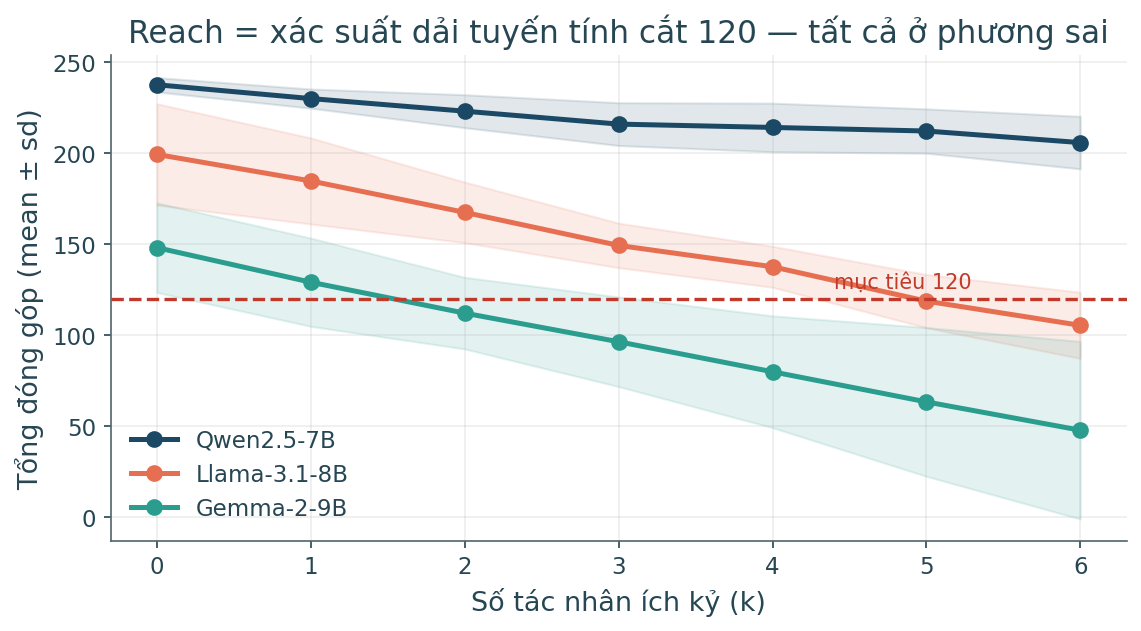
\includegraphics[height=0.66\textheight]{figs/D2_persona_dispersion.png}
  \take{Tổng đóng góp giảm tuyến tính theo $k$; đường reach kịch tính chỉ là nơi dải (mean$\pm$sd) cắt 120. Gemma ở $k{=}1$ trung bình 129 ($>$120) nhưng sd$\sim$24 cưỡi vạch $\Rightarrow$ chỉ $\sim$50\% đạt.}
\end{frame}

\begin{frame}{Persona — một động cơ tuyến tính, ba chế độ}
  \centering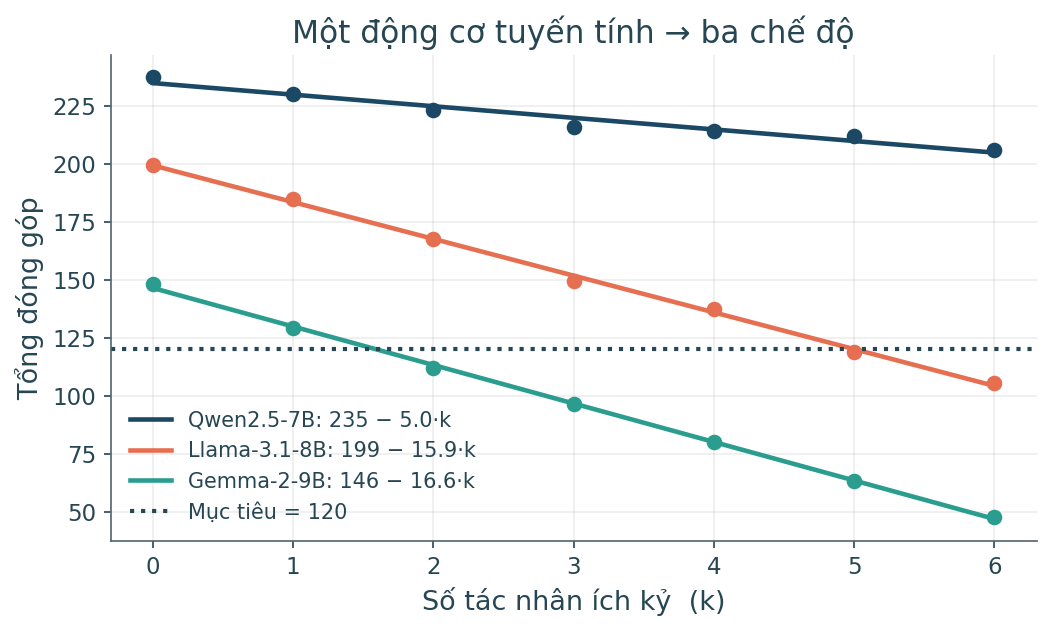
\includegraphics[height=0.66\textheight]{figs/E_persona_linear.png}
  \take{Đóng góp giảm tuyến tính theo số tác nhân ích kỷ; đường "đạt mục tiêu" kịch tính chỉ là nơi đường thẳng cắt 120.}
\end{frame}

\begin{frame}{Persona — ăn ở cấp cá nhân, nhưng Qwen ít nghe}
  \centering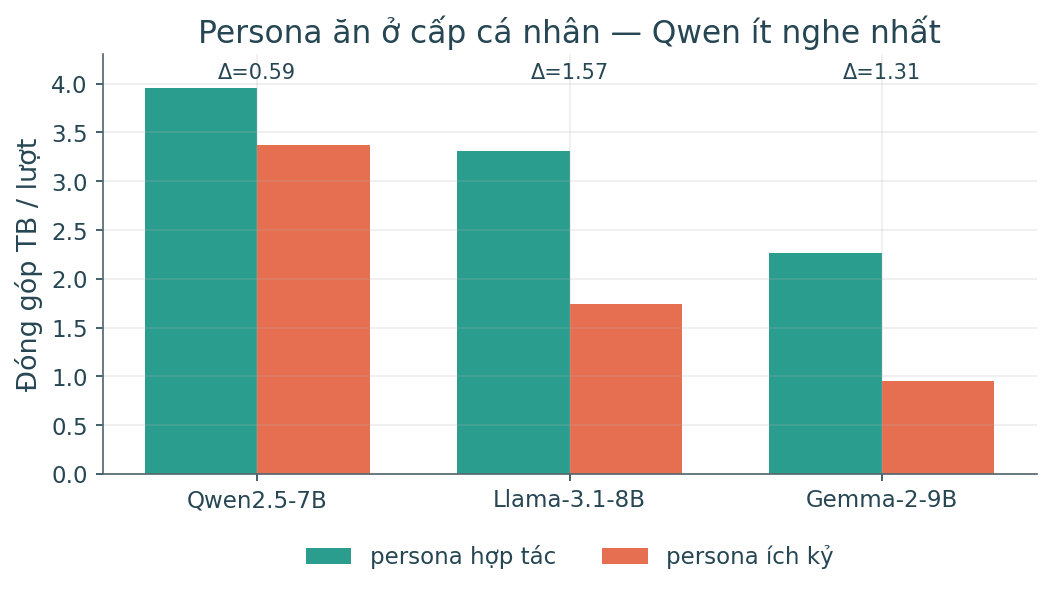
\includegraphics[height=0.64\textheight]{figs/G_disposition.png}
  \take{Tác nhân "ích kỷ" của Qwen vẫn đóng 3.4/4 ($\Delta$=0.59); Llama nghe lời rõ nhất.}
\end{frame}

\begin{frame}{Persona — sụp đổ của Gemma là do tiếng Anh}
  \centering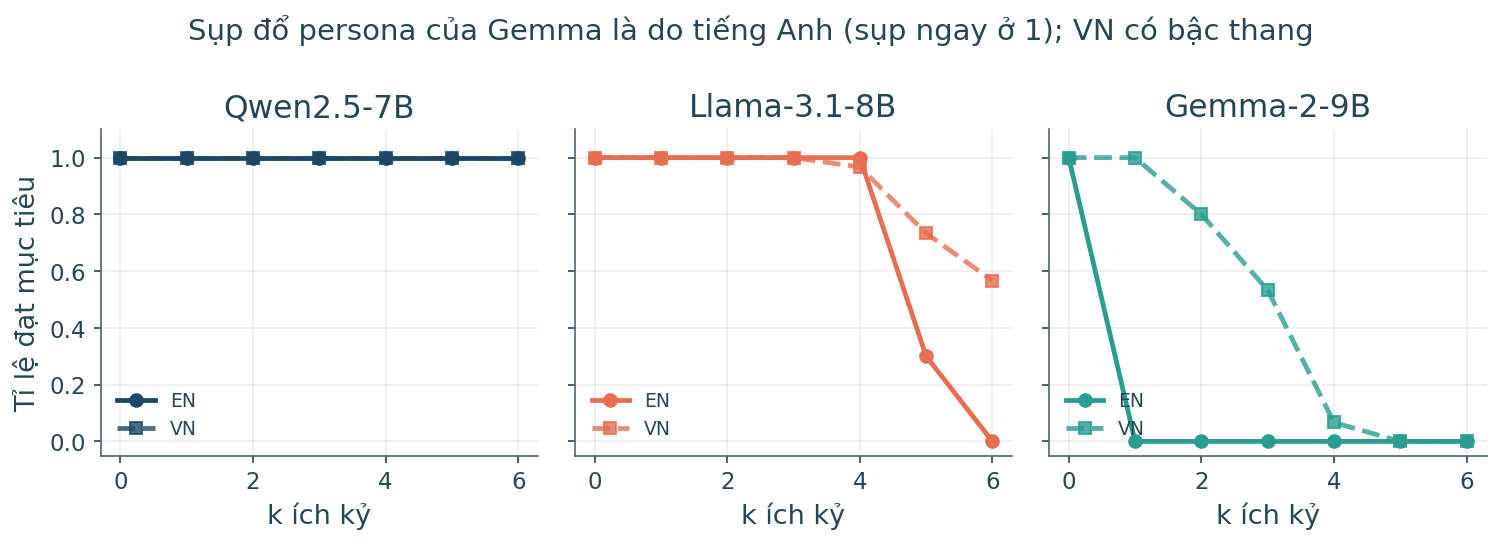
\includegraphics[height=0.62\textheight]{figs/J_persona_lang.png}
  \take{Gemma-EN: chỉ 1 ích kỷ là reach về 0\% (cooperator khoá cứng sàn 2); Gemma-VN xuống theo bậc thang (1:100\% 2:80\% 3:53\%) nhờ còn dư địa ramp cuối game. Qwen trơ ở cả hai ngôn ngữ.}
\end{frame}

\begin{frame}{Persona — kiểm chứng tính vững (vị trí ghế)}
  \centering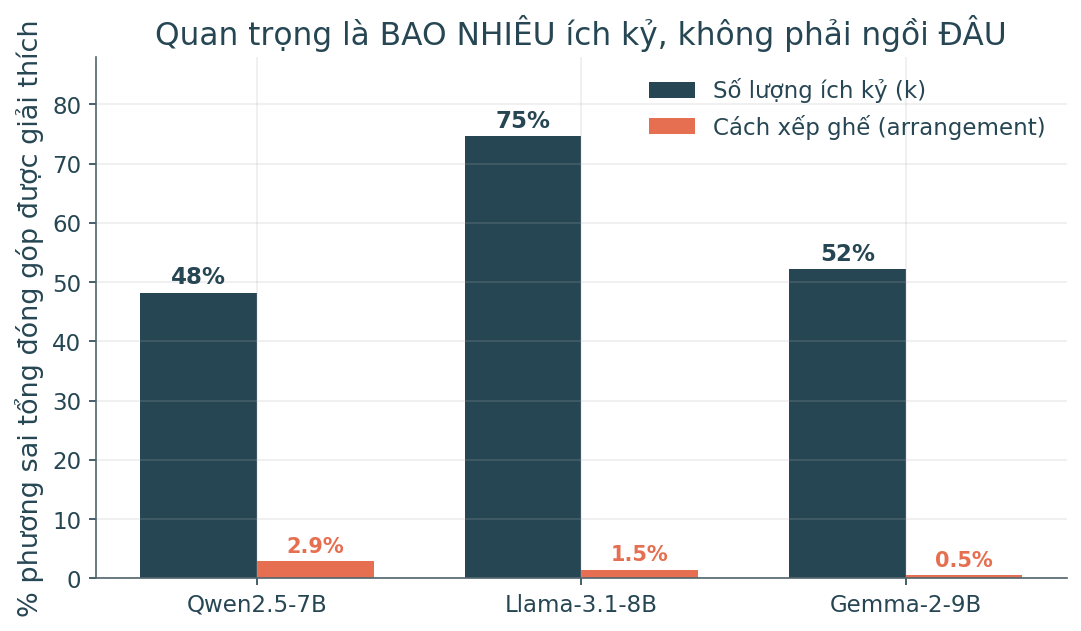
\includegraphics[height=0.64\textheight]{figs/Q_persona_variance.png}
  \take{SỐ LƯỢNG ích kỷ giải thích 48–75\% phương sai; CÁCH XẾP GHẾ chỉ 0.5–2.9\% $\Rightarrow$ dose-response không phụ thuộc vị trí. Chỉ còn “primacy” theo nhãn \texttt{Player\_1} rất nhỏ.}
\end{frame}

% ======================================================================
\section{Tổng hợp}

\begin{frame}{Hiệu quả kinh tế — ai “khôn” nhất?}
  \centering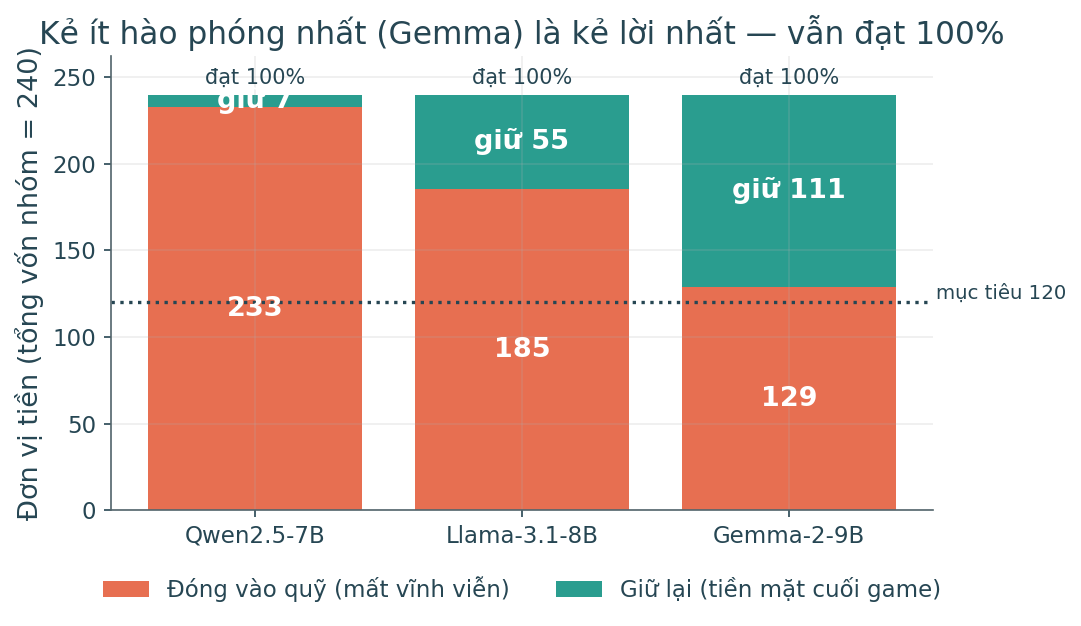
\includegraphics[height=0.64\textheight]{figs/P_efficiency.png}
  \take{Cả ba đều đạt 100\%, nhưng Gemma giữ lại 111/240 tiền mặt, Llama 55, Qwen chỉ 7 $\Rightarrow$ model “ít hào phóng” nhất lại tối ưu kinh tế nhất: đạt mục tiêu mà tốn ít nhất.}
\end{frame}

\begin{frame}{So với người: bảng tổng}
  \centering\small
  \begin{tabular}{lll}
    \toprule
    Khía cạnh & Người (Milinski 2008) & LLM (cả 3) \\
    \midrule
    Nhạy rủi ro        & Có (50/10/0\%) & \alert{Không} (100\% phẳng) \\
    Hợp tác qua vòng   & Giảm dần       & \alert{Tăng dần} \\
    Phản bội cuối game & Có             & \alert{Không} \\
    Mức đóng góp       & Vừa đủ         & \alert{Vượt mục tiêu} \\
    Phản ứng persona   & ---            & Có (mạnh nhất) \\
    \bottomrule
  \end{tabular}
  \take{LLM \emph{hợp tác hơn nhưng kém "duy lý chiến lược"} so với người.}
\end{frame}

\begin{frame}{Cơ chế sâu (đã kiểm chứng đối kháng)}
  \begin{itemize}
    \item \textbf{"Conditional cooperation" phần lớn là ảo}: sau kiểm soát trong-game, Qwen/Llama hợp tác \emph{vô điều kiện}, không theo dõi đối tác.
    \item \textbf{Cú "cứu" cuối game} của Gemma-VN là \emph{ramp theo deadline} (đóng mạnh vì game sắp hết), không phải bù trừ theo nhu cầu.
    \item \textbf{Ghi sổ sai có hệ thống}: Qwen/Llama ghi tổng chỉ $\sim$1/3 thực tế — nhưng vẫn đạt mục tiêu $\Rightarrow$ hợp tác là \emph{prior}, không phải tính toán.
    \item \textbf{Trục ngôn ngữ}: bù trừ chỉ ở VN; framing nặng hơn ở VN; persona-collapse nặng hơn ở EN.
  \end{itemize}
\end{frame}

\begin{frame}{Điểm thảo luận với thầy}
  \textbf{Về prompt}
  \begin{itemize}
    \item Khung framing lẫn confound (\emph{có} câu mục tiêu vs \emph{không}); có cần khối neutral cân bằng?
    \item Baseline (full history) khác paper — có nên lấy \emph{scratchpad} làm điều kiện chính?
  \end{itemize}
  \textbf{Về phương pháp}
  \begin{itemize}
    \item \texttt{target\_reached} bão hoà 100\% $\Rightarrow$ dùng \emph{mức đóng góp} làm biến phụ thuộc chính.
    \item Lỗi nhỏ: hoán vị ghế phủ chưa đều + "primacy" theo nhãn \texttt{Player\_1} (ảnh hưởng <3\%).
  \end{itemize}
\end{frame}

\begin{frame}[standout]
  Tác nhân LLM: kẻ \textbf{hợp tác vô điều kiện}, \textbf{phớt lờ rủi ro}, làm \textbf{ngược đường cong người} — và \textbf{ngôn ngữ} là trục điều tiết chính.
\end{frame}

\end{document}
